\let\negmedspace\undefined
\let\negthickspace\undefined
\documentclass[journal,12pt,onecolumn]{IEEEtran}
\usepackage{cite}
\usepackage{amsmath,amssymb,amsfonts,amsthm}
\usepackage{algorithmic}
\usepackage{graphicx}
\graphicspath{{./figs/}}
\usepackage{textcomp}
\usepackage{xcolor}
\usepackage{txfonts}
\usepackage{listings}
\usepackage{enumitem}
\usepackage{mathtools}
\usepackage{gensymb}
\usepackage{comment}
\usepackage{caption}
\usepackage[breaklinks=true]{hyperref}
\usepackage{tkz-euclide} 
\usepackage{listings}
\usepackage{gvv}                                        
%\def\inputGnumericTable{}                                 
\usepackage[latin1]{inputenc}     
\usepackage{xparse}
\usepackage{color}                                            
\usepackage{array}                                            
\usepackage{longtable}                                       
\usepackage{calc}                                             
\usepackage{multirow}
\usepackage{multicol}
\usepackage{hhline}                                           
\usepackage{ifthen}                                           
\usepackage{lscape}
\usepackage{tabularx}
\usepackage{array}
\usepackage{float}
\newtheorem{theorem}{Theorem}[section]
\newtheorem{problem}{Problem}
\newtheorem{proposition}{Proposition}[section]
\newtheorem{lemma}{Lemma}[section]
\newtheorem{corollary}[theorem]{Corollary}
\newtheorem{example}{Example}[section]
\newtheorem{definition}[problem]{Definition}
\newcommand{\BEQA}{\begin{eqnarray}}
\newcommand{\EEQA}{\end{eqnarray}}
\newcommand{\define}{\stackrel{\triangle}{=}}
\theoremstyle{remark}
\newtheorem{rem}{Remark}

\begin{document}
\title{
ASSIGNMENT 3: GATE 2018  \\
PI : PRODUCTION \& INDUSTRIAL ENGINEERING}
\author{EE25BTECH11054 - S. Harsha Vardhan Reddy}
\maketitle
\renewcommand{\thefigure}{\theenumi}
\renewcommand{\thetable}{\theenumi}

\begin{enumerate}

\item "The dress \underline{\hspace{2cm}} her so well that they all immediately \underline{\hspace{2cm}} her on her appearance." \par The words that best fill the blanks in the above sentence are

\hfill{\brak{\text{GATE GA 2018}}}

\begin{enumerate}
\begin{multicols}{2}
\item complemented, complemented
\item complimented, complemented
\item complimented, complimented
\item complemented, complimented
\end{multicols}
\end{enumerate}

\item "The judge's standing in the legal community, though shaken by false allegations of wrongdoing, remained \underline{\hspace{2cm}}." \par The word that best fills the blank in the above sentence is

\hfill{\brak{\text{GATE GA 2018}}}

\begin{enumerate}
\begin{multicols}{4}
\item undiminished
\item damaged
\item illegal
\item uncertain
\end{multicols}
\end{enumerate}

\item Find the missing group of letters in the following series: \par BC, FGH, LMNO, \underline{\hspace{2cm}}

\hfill{\brak{\text{GATE GA 2018}}}

\begin{enumerate}
\begin{multicols}{4}
\item UVWXY
\item TUVWX
\item STUVW
\item RSTUV
\end{multicols}
\end{enumerate}

\item The perimeters of a circle, a square and an equilateral triangle are equal. Which one of the following statements is true?

\hfill{\brak{\text{GATE GA 2018}}}

\begin{enumerate}
\begin{multicols}{2}
\item The circle has the largest area.
\item The square has the largest area.
\item The equilateral triangle has the largest area.
\item All the three shapes have the same area.
\end{multicols}
\end{enumerate}

\item The value of the expression $\frac{1}{1+\log_{u} vw} + \frac{1}{1+\log_{v} wu} + \frac{1}{1+\log_{w} uv}$ is

\hfill{\brak{\text{GATE GA 2018}}}

\begin{enumerate}
\begin{multicols}{4}
\item $-1$
\item $0$
\item $1$
\item $3$
\end{multicols}
\end{enumerate}

\item Forty students watched films A, B and C over a week. Each student watched either only one film or all three. Thirteen students watched film A, sixteen students watched film B and nineteen students watched film C. How many students watched all three films?

\hfill{\brak{\text{GATE GA 2018}}}

\begin{enumerate}
\begin{multicols}{4}
\item $0$
\item $2$
\item $4$
\item $8$
\end{multicols}
\end{enumerate}

\item A wire would enclose an area of $1936~m^2$, if it is bent into a square. The wire is cut into two pieces. The longer piece is thrice as long as the shorter piece. The long and the short pieces are bent into a square and a circle, respectively. Which of the following choices is closest to the sum of the areas enclosed by the two pieces in square meters?

\hfill{\brak{\text{GATE GA 2018}}}

\begin{enumerate}
\begin{multicols}{4}
\item $1096$
\item $1111$
\item $1243$
\item $2486$
\end{multicols}
\end{enumerate}

\item A contract is to be completed in $52$ days and $125$ identical robots were employed, each operational for $7$ hours a day. After $39$ days, five-seventh of the work was completed. How many additional robots would be required to complete the work on time, if each robot is now operational for $8$ hours a day?

\hfill{\brak{\text{GATE GA 2018}}}

\begin{enumerate}
\begin{multicols}{4}
\item $50$
\item $89$
\item $146$
\item $175$
\end{multicols}
\end{enumerate}

\item A house has a number which needs to be identified. The following three statements are given that can help in identifying the house number.
\begin{enumerate}
    \item[i.] If the house number is a multiple of $3$, then it is a number from $50$ to $59$.
    \item[ii.] If the house number is NOT a multiple of $4$, then it is a number from $60$ to $69$.
    \item[iii.] If the house number is NOT a multiple of $6$, then it is a number from $70$ to $79$.
\end{enumerate}
What is the house number?

\hfill{\brak{\text{GATE GA 2018}}}

\begin{enumerate}
\begin{multicols}{4}
\item $54$
\item $65$
\item $66$
\item $76$
\end{multicols}
\end{enumerate}

\item An unbiased coin is tossed six times in a row and four different such trials are conducted. One trial implies six tosses of the coin. If H stands for head and T stands for tail, the following are the observations from the four trials:
\begin{enumerate}
    \item[$\brak{1}$] HTHTHT
    \item[$\brak{2}$] TTHHHT
    \item[$\brak{3}$] HTTHHT
    \item[$\brak{4}$] HHHT\_\_
\end{enumerate}
Which statement describing the last two coin tosses of the fourth trial has the highest probability of being correct?

\hfill{\brak{\text{GATE GA 2018}}}

\begin{enumerate}
\item Two T will occur.
\item One H and one T will occur.
\item Two H will occur.
\item One H will be followed by one T.
\end{enumerate}
\end{enumerate}
\begin{enumerate}
\item Vector triple product $a \times \brak{b \times c}$ of three vectors a, b and c is given by

\hfill{\brak{\text{GATE PI 2018}}}

\begin{enumerate}
\begin{multicols}{2}
\item $\brak{a \bullet c}b - \brak{a \bullet b}c$
\item $\brak{b \bullet c}a - \brak{a \bullet c}b$
\item $\brak{a \bullet b}c - \brak{a \bullet c}b$
\item $\brak{b \bullet c}a - \brak{a \bullet b}c$
\end{multicols}
\end{enumerate}

\item A real-valued function y of real variable x is such that $y=5\abs{x}$. At $x=0$, the function is

\hfill{\brak{\text{GATE PI 2018}}}

\begin{enumerate}
\begin{multicols}{2}
\item discontinuous but differentiable
\item both continuous and differentiable
\item discontinuous and not differentiable
\item continuous but not differentiable
\end{multicols}
\end{enumerate}

\item Considering the coordinate system shown in the figure, a force of magnitude $10$ kN has x-component of $-6$ kN. Possible y-component\brak{s} of the force is/are
\begin{figure}[h]
    \centering
    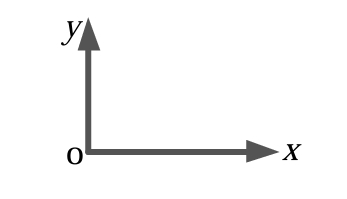
\includegraphics[width=0.2\columnwidth]{q3.png}
    \caption*{}
    \label{fig:q3}
\end{figure}

\hfill{\brak{\text{GATE PI 2018}}}

\begin{enumerate}
\begin{multicols}{2}
\item $+8$ kN only
\item $+5$ kN only
\item $+8$ kN and $-8$ kN
\item $+5$ kN and $-5$ kN
\end{multicols}
\end{enumerate}

\item When austenite decomposes upon cooling into two phases  ferrite and cementite, the reaction is called

\hfill{\brak{\text{GATE PI 2018}}}

\begin{enumerate}
\begin{multicols}{4}
\item Eutectic
\item Eutectoid
\item Peritectic
\item Peritectoid
\end{multicols}
\end{enumerate}

\item Match the geometric tolerances with their correct symbols:
\begin{table}[h]
\centering
\caption*{}
\label{tab:q5}
\begin{tabular}{llcl}
P. & Flatness & 1. & 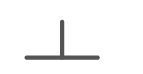
\includegraphics[height=1em]{q5_1.png} \\
Q. & Perpendicularity & 2. & 
\includegraphics[height=1em]{q5_2.png} \\
R. & Concentricity & 3. & 
\includegraphics[height=1em]{q5_3.png} \\
S. & Roundness \brak{Circularity} & 4. & 
\includegraphics[height=1em]{q5_4.png} \\
\end{tabular}
\end{table}

\hfill{\brak{\text{GATE PI 2018}}}

\begin{enumerate}
\begin{multicols}{2}
\item P-1, Q-3, R-4, S-2
\item P-3, Q-1, R-4, S-2
\item P-3, Q-1, R-2, S-4
\item P-3, Q-2, R-1, S-4
\end{multicols}
\end{enumerate}

\item Which one of the following instruments makes use of the principle of interference of light?

\hfill{\brak{\text{GATE PI 2018}}}

\begin{enumerate}
\begin{multicols}{2}
\item Optical flat
\item Auto-collimator
\item Optical projector
\item Coordinate measuring machine
\end{multicols}
\end{enumerate}

\item In ASME process chart, the symbol 
\includegraphics[height=1em]{q7.png} represents

\hfill{\brak{\text{GATE PI 2018}}}

\begin{enumerate}
\begin{multicols}{4}
\item operation
\item inspection
\item delay
\item transport
\end{multicols}
\end{enumerate}

\item Which one of the following is the most appropriate control chart for measuring the variability of individual readings within a sample?

\hfill{\brak{\text{GATE PI 2018}}}

\begin{enumerate}
\begin{multicols}{4}
\item $\bar{X}$-chart
\item R-chart
\item p-chart
\item c-chart
\end{multicols}
\end{enumerate}

\item The machines and auxiliary facilities are located according to processing sequence of the product \brak{\text{produced in very large quantities}}in

\hfill{\brak{\text{GATE PI 2018}}}

\begin{enumerate}
\begin{multicols}{2}
\item Process Layout
\item Fixed Position Layout
\item Product Layout
\item Cellular Layout
\end{multicols}
\end{enumerate}

\item Which one of the following defects is NOT associated with the casting process?

\hfill{\brak{\text{GATE PI 2018}}}

\begin{enumerate}
\begin{multicols}{4}
\item Hot tear
\item Porosity
\item Blister
\item Central burst
\end{multicols}
\end{enumerate}

\item In an oxy-acetylene gas welding process, oxygen and acetylene are mixed in a ratio of $1.5:1$ \brak{\text{by volume}}. The flame is

\hfill{\brak{\text{GATE PI 2018}}}

\begin{enumerate}
\begin{multicols}{4}
\item neutral
\item carburizing
\item reducing
\item oxidizing
\end{multicols}
\end{enumerate}

\item Each of three firms P, Q and R manufactures $100$ lakhs components. The number of defective components produced by P, Q and R are $30$, $42$ and $47$, respectively. The firm\brak{s} in conformance with Six Sigma standard is/are

\hfill{\brak{\text{GATE PI 2018}}}

\begin{enumerate}
\begin{multicols}{4}
\item only P
\item P and Q
\item P, Q and R
\item Q and R
\end{multicols}
\end{enumerate}

\item To make holes of $0.5$ mm diameter and $30$ mm depth in a mild steel component, the most suitable process is

\hfill{\brak{\text{GATE PI 2018}}}

\begin{enumerate}
\begin{multicols}{2}
\item chemical machining
\item electrochemical machining
\item abrasive jet machining
\item plasma arc machining
\end{multicols}
\end{enumerate}

\item Which one of the following processes is NOT used for producing powders?

\hfill{\brak{\text{GATE PI 2018}}}

\begin{enumerate}
\begin{multicols}{4}
\item Atomization
\item Ball milling
\item Sintering
\item Electrolysis
\end{multicols}
\end{enumerate}

\item The process in which molten thermoplastic is forced between rolls to produce thin sheets is called

\hfill{\brak{\text{GATE PI 2018}}}

\begin{enumerate}
\begin{multicols}{2}
\item blow moulding
\item compression moulding
\item calendering
\item extrusion
\end{multicols}
\end{enumerate}

\item The diagonal elements of a 3-by-3 matrix are $-10$, $5$ and $0$, respectively. If two of its eigenvalues are $-15$ each, the third eigenvalue is \underline{\hspace{2cm}}.

\hfill{\brak{\text{GATE PI 2018}}}

\item Weights \brak{\text{in kg}} of six products are $3$, $7$, $6$, $2$, $3$ and $4$. The median weight \brak{\text{in kg, up to one decimal place}} is \underline{\hspace{2cm}}.

\hfill{\brak{\text{GATE PI 2018}}}

\item The probabilities of occurrence of events F and G are $P\brak{F}=0.3$ and $P\brak{G}=0.4$, respectively. The probability that both events occur simultaneously is $P\brak{F \cap G}=0.2$. The probability of occurrence of at least one event $P\brak{F \cup G}$ is \underline{\hspace{2cm}}.

\hfill{\brak{\text{GATE PI 2018}}}

\item A flywheel in the form of a solid circular disc of radius $100$ mm and uniform thickness has a mass of $10$ kg. If it is rotating at a uniform angular velocity of $20~\text{rad/s}$, the kinetic energy \brak{\text{in J}} of the flywheel is \underline{\hspace{2cm}}.

\hfill{\brak{\text{GATE PI 2018}}}

\item A cylindrical wooden block of length $50$ cm is floating in water in such a way that its axis is vertical. The densities of wood and water are $800~\text{kg/m}^3$ and $1000~\text{kg/m}^3$, respectively. The submerged depth, i.e., depth of immersion \brak{\text{in cm}}1 of the cylinder is \underline{\hspace{2cm}}.

\hfill{\brak{\text{GATE PI 2018}}}

\item A machine consists of three components P, Q and R connected serially. The reliabilities of P, Q and R are $0.97$, $0.86$ and $0.93$, respectively. To increase the reliability of the machine, two additional stand-by units of Q are attached. The overall reliability \brak{\text{up to two decimal places}} of the machine is \underline{\hspace{2cm}}.

\hfill{\brak{\text{GATE PI 2018}}}

\item The mean time between failures of a machine is $400$ hour. If the availability of the machine is $80\%$, the mean time to repair \brak{\text{in hour}} is \underline{\hspace{2cm}}.

\hfill{\brak{\text{GATE PI 2018}}}

\item Processing times on a single machine for $3$ jobs are given below. All the jobs are available at time $t=0$.
\begin{table}[h]
    \centering
    \caption*{}
    \label{tab:q23}
    \begin{tabular}{|l|c|c|c|}
    \hline
    \textbf{Job} & 1 & 2 & 3 \\
    \hline
    \textbf{Processing time \brak{minute}} & 15 & 3 & 6 \\
    \hline
    \end{tabular}
\end{table}
The mean flow time \brak{\text{in minute}}   as per the shortest processing time \brak{SPT} sequence is \underline{\hspace{2cm}}.

\hfill{\brak{\text{GATE PI 2018}}}

\item In a two-pass wire drawing process, there is a $40\%$ reduction in wire cross-sectional area in $1^{st}$ pass and further $30\%$ reduction in 2nd pass. The overall reduction \brak{in percentage} is \underline{\hspace{2cm}}.

\hfill{\brak{\text{GATE PI 2018}}}

\item A double-start thread with a pitch of $2$ mm is to be cut using a lathe machine. The pitch of the leadscrew of the lathe is $6$ mm. The job rotates at $60$ revolution per minute \brak{RPM}. The RPM of the leadscrew is \underline{\hspace{2cm}}.

\hfill{\brak{\text{GATE PI 2018}}}

\item Consider the analytic function $f\brak{z}=x^2 - y^2 + i2xy$ of the complex variable $z=x+iy$, where $i=\sqrt{-1}$. The derivative $f'\brak{z}$ is

\hfill{\brak{\text{GATE PI 2018}}}

\begin{enumerate}
\begin{multicols}{4}
\item $2x+i2y$
\item $x^2 + iy^2$
\item $x+iy$
\item $2x-i2y$
\end{multicols}
\end{enumerate}

\item In order to evaluate the integral $\int e^x dx$ with Simpson's $1/3^{rd}$ rule, values of the function $e^x$ are used at $x=0.0, 0.5$ and $1.0$. The absolute value of the error of numerical integration is

\hfill{\brak{\text{GATE PI 2018}}}

\begin{enumerate}
\begin{multicols}{4}
\item $0.000171$
\item $0.000440$
\item $0.000579$
\item $0.002718$
\end{multicols}
\end{enumerate}

\item A rigid link PQ of length $1.0$ m is pinned at P. It rotates about P in a vertical plane with a uniform angular acceleration of $1.0~\text{rad/s}^2$. At an instant when the angular velocity of the link is $1.0~\text{rad/s}$ the magnitude of total acceleration \brak{\text{in m/s$^2$}} of point Q relative to point P is

\hfill{\brak{\text{GATE PI 2018}}}

\begin{enumerate}
\begin{multicols}{4}
\item $1.41$
\item $1.73$
\item $2$
\item $2.83$
\end{multicols}
\end{enumerate}

\item In a shaft-hole system, the dimensions with tolerances \brak{in mm} are as follows:
Shaft: $\phi 20_{-x}^{+x}$ \quad Hole: $\phi 20_{-y}^{-0.03}$
where both x and y are positive real numbers. Which one of the following will provide an interference fit?

\hfill{\brak{\text{GATE PI 2018}}}

\begin{enumerate}
\begin{multicols}{2}
\item $x=0.05, y=0.040$
\item $x=0.04, y=0.035$
\item $x=0.04, y=0.032$
\item $x=0.02, y=0.035$
\end{multicols}
\end{enumerate}

\item A machine is procured at a price of Rs. $47000$ with a 2-year warranty. After two years, the annual maintenance cost \brak{AMC} in Rs. is given by the following formula:
$AMC=\brak{i-2} \times 2000$, for $i>2$,
where i is the number of years elapsed since the machine was purchased. Neglect the scrap value of the machine, inflation, interest, etc. For minimizing the average cost, the machine should be replaced at the end of the year

\hfill{\brak{\text{GATE PI 2018}}}

\begin{enumerate}
\begin{multicols}{4}
\item $2$
\item $4$
\item $7$
\item $10$
\end{multicols}
\end{enumerate}

\item In a service centre, cars arrive according to Poisson distribution with a mean of $2$ cars per hour. The time for servicing a car is exponential with a mean of $15$ minutes. The expected waiting time \brak{in minute} in the queue is

\hfill{\brak{\text{GATE PI 2018}}}

\begin{enumerate}
\begin{multicols}{4}
\item $10$
\item $15$
\item $25$
\item $30$
\end{multicols}
\end{enumerate}

\item Actual and forecasted demands of a product are as follows:
\begin{table}[h]
    \centering
    \caption*{}
    \label{tab:q32}
    \begin{tabular}{|l|c|c|c|c|c|}
    \hline
    \textbf{Period} & 1 & 2 & 3 & 4 & 5 \\
    \hline
    \textbf{Actual demand} & 180 & 170 & 165 & 170 & 200 \\
    \hline
    \textbf{Forecasted demand} & 190 & 190 & 190 & 190 & 190 \\
    \hline
    \end{tabular}
\end{table}
The forecast error measured in terms of mean absolute deviation \brak{MAD} and mean absolute percentage error \brak{MAPE}, respectively, are

\hfill{\brak{\text{GATE PI 2018}}}

\begin{enumerate}
\begin{multicols}{4}
\item $13$ and $7.84\%$
\item $13$ and $9.85\%$
\item $17$ and $7.84\%$
\item $17$ and $9.85\%$
\end{multicols}
\end{enumerate}

\item In a mass production firm, measurements are carried out on $10000$ pairs of shaft and hole. The mean diameters of the shaft and the hole are $37.53$ mm and $37.59$ mm, respectively. The corresponding standard deviations are $0.03$ mm and $0.04$ mm. The mean clearance and its standard deviation \brak{\text{both in mm}}, respectively, are

\hfill{\brak{\text{GATE PI 2018}}}

\begin{enumerate}
\begin{multicols}{4}
\item $0.06$ and $0.07$
\item $0.06$ and $0.06$
\item $0.06$ and $0.05$
\item $0.07$ and $0.01$
\end{multicols}
\end{enumerate}

\item A pressure die casting set-up was tested by injecting water \brak{\text{density 1000 kg/m$^3$}} at a pressure of $200$ bar. Mould-filling time was found to be $0.05$ s. Afterwards, the actual casting is made by injecting the liquid metal \brak{\text{density 2000 kg/m$^3$}} at an injection pressure of $400$ bar. Neglect all losses \brak{friction, viscous-effect, etc.}. The approximate mould-filling time  \brak{\text{in s}} is

\hfill{\brak{\text{GATE PI 2018}}}

\begin{enumerate}
\begin{multicols}{4}
\item $0.05$
\item $0.075$
\item $0.1$
\item $0.2$
\end{multicols}
\end{enumerate}

\item The value of the surface integral $\iint_S \brak{9x\mathbf{i} - 2y\mathbf{j} - z\mathbf{k}} \cdot \mathbf{n} dS$ over the surface S of the sphere $x^2 + y^2 + z^2 = 9$, where n is the unit outward normal to the surface element dS, is \underline{\hspace{2cm}}.

\hfill{\brak{\text{GATE PI 2018}}}

\item Consider the differential equation $2\frac{d^2y}{dt^2} + 8y = 0$ with initial conditions: at $t=0, y=0$ and $\frac{dy}{dt}=10$. The value of y \brak{\text{up to two decimal places}} at $t=1$ is \underline{\hspace{2cm}}.

\hfill{\brak{\text{GATE PI 2018}}}

\item One kg of air\brak{\text {that can be considered a calorically perfect gas with characteristic gas constant 
$R = 287 \,\text{J/kg-K}$ and specific heat ratio $\gamma = 1.4$ }} undergoes a constant-volume process from an initial static pressure of $1$ bar to a final static pressure of $4$ bar. The increase in entropy \brak{\text{in J/kg-K}}of air is \underline{\hspace{2cm}}.

\hfill{\brak{\text{GATE PI 2018}}}

\item If $u = 2\brak{x^2 - y^2}$ and $v = -axy$ represent the x- and y-components of the two-dimensional velocity field of an incompressible flow, the value of the constant a is \underline{\hspace{2cm}}.

\hfill{\brak{\text{GATE PI 2018}}}

\item A spherical pressure vessel \brak{made of mild steel} of internal diameter $500$ mm and thickness $10$ mm is subjected to an internal gauge pressure of $4000$ kPa. If the yield stress of mild steel is $200$ MPa, the factor of safety \brak{\text{up to one decimal place}} is \underline{\hspace{2cm}}.

\hfill{\brak{\text{GATE PI 2018}}}

\item A square cross-section wooden column of length $3140$ mm is pinned at both ends. For the wood, Young's modulus of elasticity is $12$ GPa and allowable compressive stress is $12$ MPa. The column needs to support an axial compressive load of $200$ kN. Using a factor of safety of $2.0$ in the computation of Euler's buckling load, the minimum cross-sectional area \brak{\text{in mm$^2$}}of the column is \underline{\hspace{2cm}}.

\hfill{\brak{\text{GATE PI 2018}}}

\item Length, width and thickness of a plate are $400$ mm, $400$ mm and $30$ mm, respectively. For the material of the plate, Young's modulus of elasticity is $70$ GPa, yield stress is $80$ MPa and Poisson's ratio is $0.33$. When the plate is subjected to a longitudinal tensile stress of $70$ MPa, the increase in the volume \brak{\text{in mm$^3$}}of the plate is \underline{\hspace{2cm}}.

\hfill{\brak{\text{GATE PI 2018}}}

\item In a V-thread, a wire is fitted such that it makes contact with the flank of the thread on the pitch line as shown in the figure. If the pitch p of the thread is $3$ mm and the included angle is $60\degree$, the diameter \brak{\text {in mm, up to one decimal place}}of the wire is \underline{\hspace{2cm}}.
\begin{figure}[h]
    \centering
    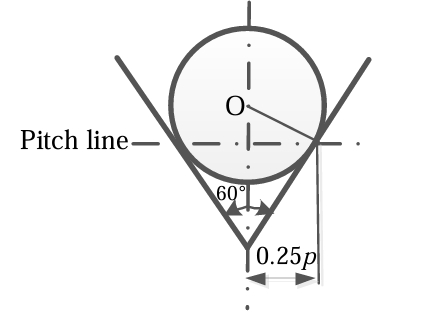
\includegraphics[width=0.3\columnwidth]{q42.png}
    \caption*{}
    \label{fig:q42}
\end{figure}

\hfill{\brak{\text{GATE PI 2018}}}

\item A project consists of three activities P, Q and R. The durations of activities follow Beta distribution. The predecessors and durations of activities are as per the following table:
\begin{table}[h]
    \centering
    \caption*{}
    \label{tab:q43}
    \begin{tabular}{|l|c|c|c|c|}
    \hline
    \textbf{Activity} & \textbf{Predecessors} & \textbf{Optimistic time \brak{month}} & \textbf{Most likely time \brak{month}} & \textbf{Pessimistic time \brak{month}} \\
    \hline
    P & --- & 2 & 3 & 10 \\
    \hline
    Q & P & 3 & 5 & 13 \\
    \hline
    R & Q & 3 & 4 & 5 \\
    \hline
    \end{tabular}
\end{table}
The expected project completion time \brak{\text {in month}} is \underline{\hspace{2cm}}.
\hfill{\brak{\text{GATE PI 2018}}}


\item A company has two manufacturing plants \brak{\text{C1 and C2}} and two distribution centres \brak{\text{D1 and D2}}. The capacities of C1 and C2 are $100$ and $200$ units, respectively. The demand for D1 and D2 are $190$ and $110$ units, respectively. The costs per unit \brak{\text{in Rs.}} of transportation at different routes are as per the following matrix:
\begin{table}[h!]
\centering
\begin{tabular}{|c|c|c|}
\hline
 & $D_1$ & $D_2$ \\ \hline
$C_1$ & 22 & 21 \\ \hline
$C_2$ & 20 & 27 \\ \hline
\end{tabular}
\end{table}
The minimum total cost \brak{\text{in Rs.}} of transportation is \underline{\hspace{2cm}}.

\hfill{\brak{\text{GATE PI 2018}}}

\item The annual demand of an item is $19845$ units and the production rate is $100$ units per day. The per-unit production cost \brak{\text{excluding setup cost}} is Rs. $50$, the per-unit holding cost is Rs. $10$ per year and setup cost is Rs. $520$ per setup. To minimize the total annual cost, the optimum quantity to be produced per setup is \underline{\hspace{2cm}}.

\hfill{\brak{\text{GATE PI 2018}}}

\item A production line operates $7$ hours a day in a 5-day week. The processing times for various job elements are as follows:
\begin{table}[h]
    \centering
    \caption*{}
    \label{tab:q46}
    \begin{tabular}{|l|c|c|c|c|c|}
    \hline
    \textbf{Job element} & p & q & r & s & t \\
    \hline
    \textbf{Processing time \brak{s}} & 5 & 10 & 12 & 3 & 15 \\
    \hline
    \end{tabular}
\end{table}
If the line is designed for an output of $8400$ units per week, the theoretical minimum number of work stations required is \underline{\hspace{2cm}}.

\hfill{\brak{\text{GATE PI 2018}}}

\item In a work sampling study of a worker, the information available are as follows: total time of study: $30$ hour, number of items produced: $320$, total number of observations: $1000$, number of observations when worker is found working: $850$ and average performance rating: $105\%$. Company policy is to give allowance of $10\%$ of total time on the job. The standard time \brak{\text{in minute per item, up to one decimal place}} for manufacturing the item is \underline{\hspace{2cm}}.

\hfill{\brak{\text{GATE PI 2018}}}

\item The breakeven point of a manufacturing company is $50000$ units. The fixed cost is Rs. $200000$ and the variable cost per unit is Rs. $20$. The selling price per unit \brak{\text{in Rs.}} of the product at this breakeven point is \underline{\hspace{2cm}}.

\hfill{\brak{\text{GATE PI 2018}}}

\item A $10$ mm thick plate is rolled to $7$ mm thickness in a rolling mill using $1000$ mm diameter rigid rolls. The neutral point is located at an angle of $0.3$ times the bite angle from the exit. The thickness \brak{\text{in mm, up to two decimal places}} of the plate at the neutral point is \underline{\hspace{2cm}}.

\hfill{\brak{\text{GATE PI 2018}}}

\item A cylindrical workpiece is turned at a feed of $0.1 \,\text{mm/rev}$ with a perfectly sharp tool. 
In ASA system, the side and end cutting edge angles are $15^\circ$ and $5^\circ$, respectively, 
as shown in the figure. 
The peak-to-valley roughness \brak{\text{in $\mu$m, up to one decimal place}}of the machined surface is \underline{\hspace{2cm}}.

\begin{figure}[H]
    \centering
    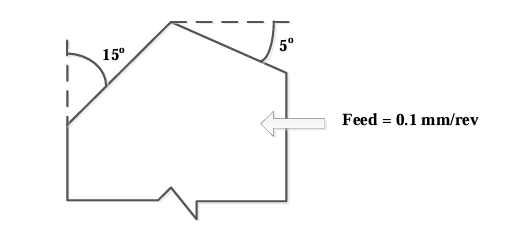
\includegraphics[width=0.4\columnwidth]{q50.png}
    \caption*{}
    \label{fig:q50}
\end{figure}

\hfill{\brak{\text{GATE PI 2018}}}

\item The worktable in a CNC machine is driven by a leadscrew with a pitch of $2$ mm. The leadscrew is directly coupled to a stepper motor of step angle $1.8\degree$. The number of pulses required to move the worktable by $50$ mm is \underline{\hspace{2cm}}.

\hfill{\brak{\text{GATE PI 2018}}}

\item During orthogonal machining of a job at a cutting speed of $90$ m/min with a tool of $10\degree$ rake angle, the cutting force and thrust force are $750$ N and $390$ N, respectively. Assume a shear angle of $35\degree$. The power \brak{\text{in W}} expended for shearing along the shear plane is \underline{\hspace{2cm}}.

\hfill{\brak{\text{GATE PI 2018}}}

\item In an electrochemical machining of aluminium with plane parallel electrodes, the current density is $70~\text{A/cm}^2$. Cross-sectional area of each electrode is $3~\text{cm}^2$ .
 The current efficiency \brak{\text{i.e., the fraction of current used for dissolution of metal}} is $80\%$. Gram atomic weight, valency and density of aluminium are $27$ gram, $3$ and $2700~\text{kg/m}^3$, respectively. Take Faraday's constant as $96500$ Coulomb. The volumetric material removal rate \brak{\text{in mm$^3$/min}} is \underline{\hspace{2cm}}.

\hfill{\brak{\text{GATE PI 2018}}}

\item Two metallic sheets are spot welded by passing a current of $8000$ A for $0.2$ s. Assume that a cylindrical nugget of $8$ mm diameter and $3$ mm depth is formed. The density of the nugget is $7500~\text{kg/m}^3$, effective resistance of the total system is $222$ micro-Ohm and heat required to produce $1.0$ gram of nugget is $1400$ J. The percentage of heat actually utilized in producing the nugget is \underline{\hspace{2cm}}.

\hfill{\brak{\text{GATE PI 2018}}}

\item In a planar 2-degree-of-freedom robot, Link 1 of $30$ cm length is connected to base by a revolute joint and Link 2 of length $20$ cm is connected to Link 1 with a revolute joint as shown in the figure. The work-envelope area \brak{\text{in cm$^2$}}, covered by point P, is \underline{\hspace{2cm}}.
\begin{figure}[h]
    \centering
    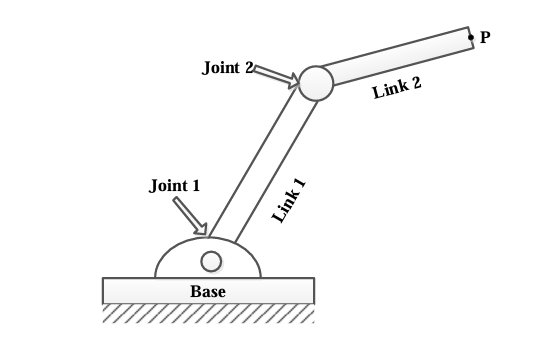
\includegraphics[width=0.3\columnwidth]{q55.png}
    \caption*{}
    \label{fig:q55}
\end{figure}

\hfill{\brak{\text{GATE PI 2018}}}

\end{enumerate}

\end{document}